%Section 3: How PET/CT overcomes those challenges (physics and technical focus).
\begin{multicols}{2}

\subsection{Technical Principles of PET/CT}


Positron Emission Tomography (PET) is a functional imaging modality that uses positron-emitting radionuclides to map metabolic activity in tissues. As standalone imaging modality it lacks of anatomic structure localization, for that it is integrated with Computed Tomography (CT). CT contribution is huge, it provides attenuation correction, electron density, and anatomical localization. This way, PET/CT provides both functional and structural data in a single imaging session and with it a valuable approach in planing and diagnosing. With the use of PET annihilation gamma rays and CT high resolution it is possible to find accurately the localization of metabolic abnormalities \cite{TG174}. By taking the best of both modalities it is ensured that all metabolic information is properly contextualized on the anatomy reducing errors on registration state compared to standalone systems \cite{TG126}.

As indicated to regular patients the protocol runs as follows, a CT scan is performed first for anatomical information and attenuation correction, then the tracer is injected intravenously. Followed by a waiting period of 30-60 minutes for tracer distribution (uptake), finally the PET scan lasts around 20-30 minutes. This paper will explore the main techincal characteristics of this general protocol.

%Why addition CT
% Resolution required?

In terms of the CT scan, a pancreas-specific protocol designed to assess pancreatic cancer employs a thin-section, multi-phase technique, which includes pre-contrast images, early arterial phase images (17-25 seconds post-contrast injection), pancreatic phase images (35-50 seconds post-injection), and portal venous phase images (55-70 seconds post-injection) \cite{Lee2014}. High-resolution CT imaging for pancreatic evaluations typically utilizes multi-detector row scanners with a minimum of four detector rows and employs thin slices (as small as 1 mm) and low tube voltages (e.g., 80 kVp or standard 120 kVp) to enhance visualization of subtle anatomical features \cite{Lee2023}. Figure \ref{fig:pancreatic_mass} illustrates an example of a MDCT image of a 64-year-old male with biopsy-proven pancreatic adenocarcinoma with liver metastasis. The pancreatic tail mass (arrow) shows isoattenuation, that is appears to have the same density or brightness as the surrounding tissue, causing distal parenchyma atrophy, meaning that the tissue further away from the mass has shrunk or wasted away \cite{Lee2014}. Imaging acquisition parameters were not disclosed.


Now on the PET technology, the most commonly used radioisotope is fluorine-18 (18F) (half-life, 110 min), which is typically attached to fluorodeoxyglucose (FDG). When this radioisotope decays, it emits a positron that travels a short distance (1-2 mm) before interacting with an electron. Then, the positron-electron interaction results in annihilation, producing two high-energy photons (511 keV each) that travel in opposite directions. These photons are detected by the PET scanner's ring of detectors, allowing for the localization of the decay event \cite{Vaquero2015}. 


In AAPM slides from a 2008 summer program given by David W Townsend PhD, a PET/CT scanner configuration is given. The PET Component has multiple rings of detectors that surround the patient. These detetors use as scintillator materials BGO, GSO, LSO, or LYSO2 and usually sizes 4x4 mm or 6x6 mm \cite{Townsend2008}.  
The field of view is characterized as 15 to 22 cm axial and 55-60 cm transaxial. With axial being increased in recent studies to 25 cm.
New developments in material science has allowed, advanced cristals, digital detectors and smaller designs with overall  sensitivity of 10\% \cite{Jones2017}.

\end{multicols}

\begin{figure}[H]
	\centering
	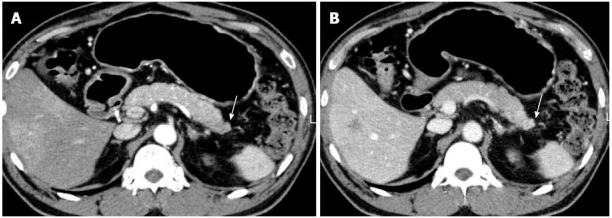
\includegraphics[width=0.95\textwidth]{assets/WJG-20-7864-g003.jpg}
	\caption{Pancreatic tail mass on Multi-Detector Computed Tomography (MDCT).\cite{Lee2014}}
	\label{fig:pancreatic_mass}
\end{figure}
 
%Physics of PET/CT
%how is this acomplished
% scanner config
%technical details
%why both

\begin{multicols}{2}
	
On the CT component end, the X-ray tube rotates around the patient and the detector array is opposite to the X-ray tube capturing the transmitted rays. A common rotation speed is 0.3-2.0 seconds and the slices go from 4 to 64 slices or more. This CT scanner is typically combined in the same device hence the name PET/CT, and features a patient port, typically 70 cm in diameter, and the gantry dimensions are approximately 228 cm x 200 cm x 168 cm \cite{Townsend2008}. Figure \ref{fig:PETCTtable} depics a typical combined device.

\begin{figure}[H]
	\centering
	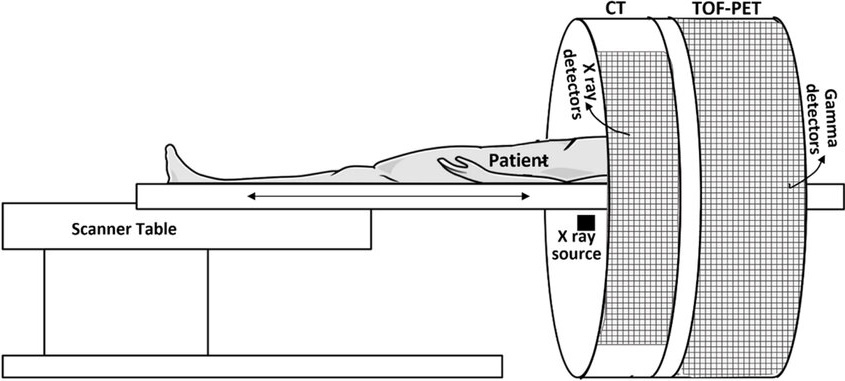
\includegraphics[width=0.45\textwidth]{assets/PETCTtable.jpg} 
	\caption{Schematic representation of TOF-capable PET/CT scanner with operational depiction of individual. Adapeted from Mohammadi \cite{figPETCT}}
	\label{fig:PETCTtable} 
\end{figure}

The spatial resolution of PET is limited by multiple factors, including the physics of positron emission, annihilation event localization, and detector technology. For exapmle, typical clinical systems achieve a spatial resolution of 4-5 mm at best, though practical imaging often operates closer to 10 mm resolution \cite{Wang2018}. And contrast in PET imaging is dependent on the radiotracer uptake, with image quality influenced by the signal-to-noise ratio, tracer concentration, and the ability to distinguish subtle metabolic differences between normal and pathological tissues \cite{Moses2011}.

The now well established Time-of-flight (TOF) technology allows to get precise timing of gamma-ray detection to improve spatial resolution and reduce noise. Initially introduced with timing resolutions around 650 picoseconds, modern digital TOF-PET systems have dramatically improved to 320 picoseconds \cite{Walrand2018}. Now, it solves the problem of presicion on measurement of the exact site of anihilation and it enchances signal-to-noise ratio (SNR), particularly for larger patients \cite{Seifert2022}. PET technology has advanced a lot in recent years with detection enhancement, such as the adoption of Silicon Photomultiplier Arrays (SiPM) replacing older photomultiplier tubes (PMTs) augment resolution and sensitivity \cite{SunderlandSeminar}.

With these advancements, the regulations and quality assessments ensure that metrics like Standardized Uptake Value (SUV) are reliable.\cite{TG174}. Daily quality checks include blank scans and visual inspections as well as regular calibration and normalization of both PET and CT components

Additionally, there is another important factor related to PET scanners, as PET imaging requires administration of radiopharmaceuticals. This administration must be performed with accuracy as any error in this step, can lead to uneven tracer distribution. The next section will explore more about the particular radiotracer [18F]FDG. Sunderland et al. demonstrated that injection infiltration occurs in less than 0.4\% of cases. Moreover, computational modeling suggests that even when infiltration occurs, its impact on dosimetry and image quality is negligible  \cite{Sunderland2023}. 




\subsection{Mechanism of [18F]FDG Uptake}


Fluorine-18 Fluorodeoxyglucose or [18F]FDG is a glucose analog labeled with the positron-emitting isotope fluorine-18. After intravenous injection, FDG is transported into cells by glucose transporters like GLUT1 and  the enzyme hexokinase adds a phosphate group (phosphorylase) to it. Since this is now a different molecule from glucose cells cannot longer proceed in the glycolysis process, and the molecule gets trapped in cells with high glucose metabolism, such as tumor cells \cite{TG174,Zheng2018}.

This characteristic of the cancer cell is what allows for PET to visualize regions of hyperglycolysis. For example, in Figure \ref{fig:PuFig1} we see a PET image on A) that show regions of increased metabolic activity in the pancreatic head, although it has poor resolution (not disclosed) it exemplifies a typical axial view of the abdominal area where the black dots indicate concentration of FDG uptake in that section. In the middle image B) a CT image provide anatomical context, this is helpful for localization of the hotspots.  The fused PET/CT image C) integrates these modalities, and allows for precise localization of pancreatic tumors.


Then oncogenic mutations like KRAS drive this process by upregulating GLUT1 and hexokinase-2, further amplifying glucose uptake \cite{Deng2021}. But this is not the only reason FDG accumlation can increase, this behaivior is also present in inflammation and benign conditions, such as autoimmune pancreatitis \cite{Zheng2018}. Different radiotracers may shine some light into the problems faced right now and and with them new advancements in tracer specificity and imaging protocols emerge.

\end{multicols}

\begin{figure}[H]
	\centering
	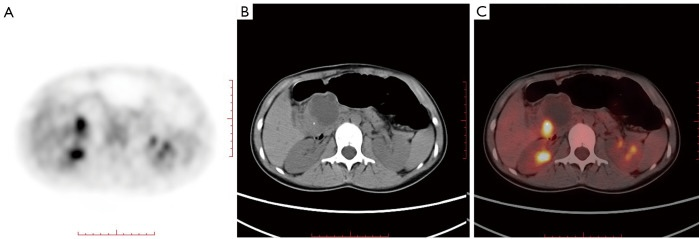
\includegraphics[width=0.95\textwidth]{assets/tcr-10-07-3560-f1.jpg}
	\caption{18F-FDG PET/CT imaging integrating metabolic and anatomical data: (A) PET image, (B) non-enhanced CT image, (C) fused PET and CT images, demonstrating pancreatic head cancer detection \cite{Pu2021}.}
	\label{fig:PuFig1}
\end{figure}


%\subsection{General Protocol for FDG PET/CT}